
\subsubsection{Estudo dos dados}

Os dados que nos propomos a prever são os de Energia Usada na Banda de Reserva Secundária, tanto a subir como a descer: "\textit{UpwardUsedSecondaryReserveEnergy}","\textit{DownwardUsedSecondaryReserveEnergy}".\par



\begin{figure}[H]
  \centering
  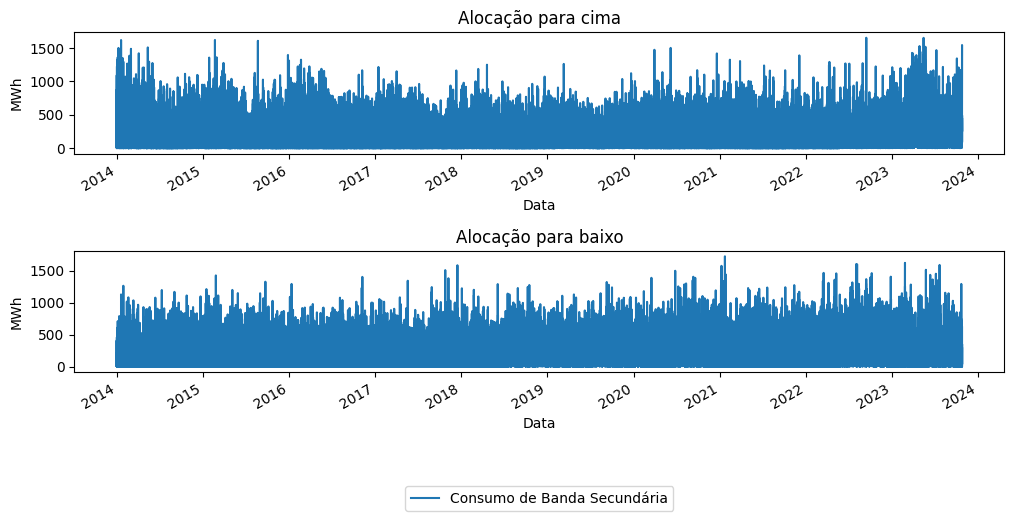
\includegraphics[width=0.6\textwidth]{plots/consumo_originais.png}
  \caption{Série Temporal dos dados alvo}
  \label{fig:targettimeseries}
\end{figure}


Para termos uma melhor percepção dos mesmos seguem, \text{infra}, quatro janelas temporais mais pequenas.

\begin{figure}[H]
  \centering
  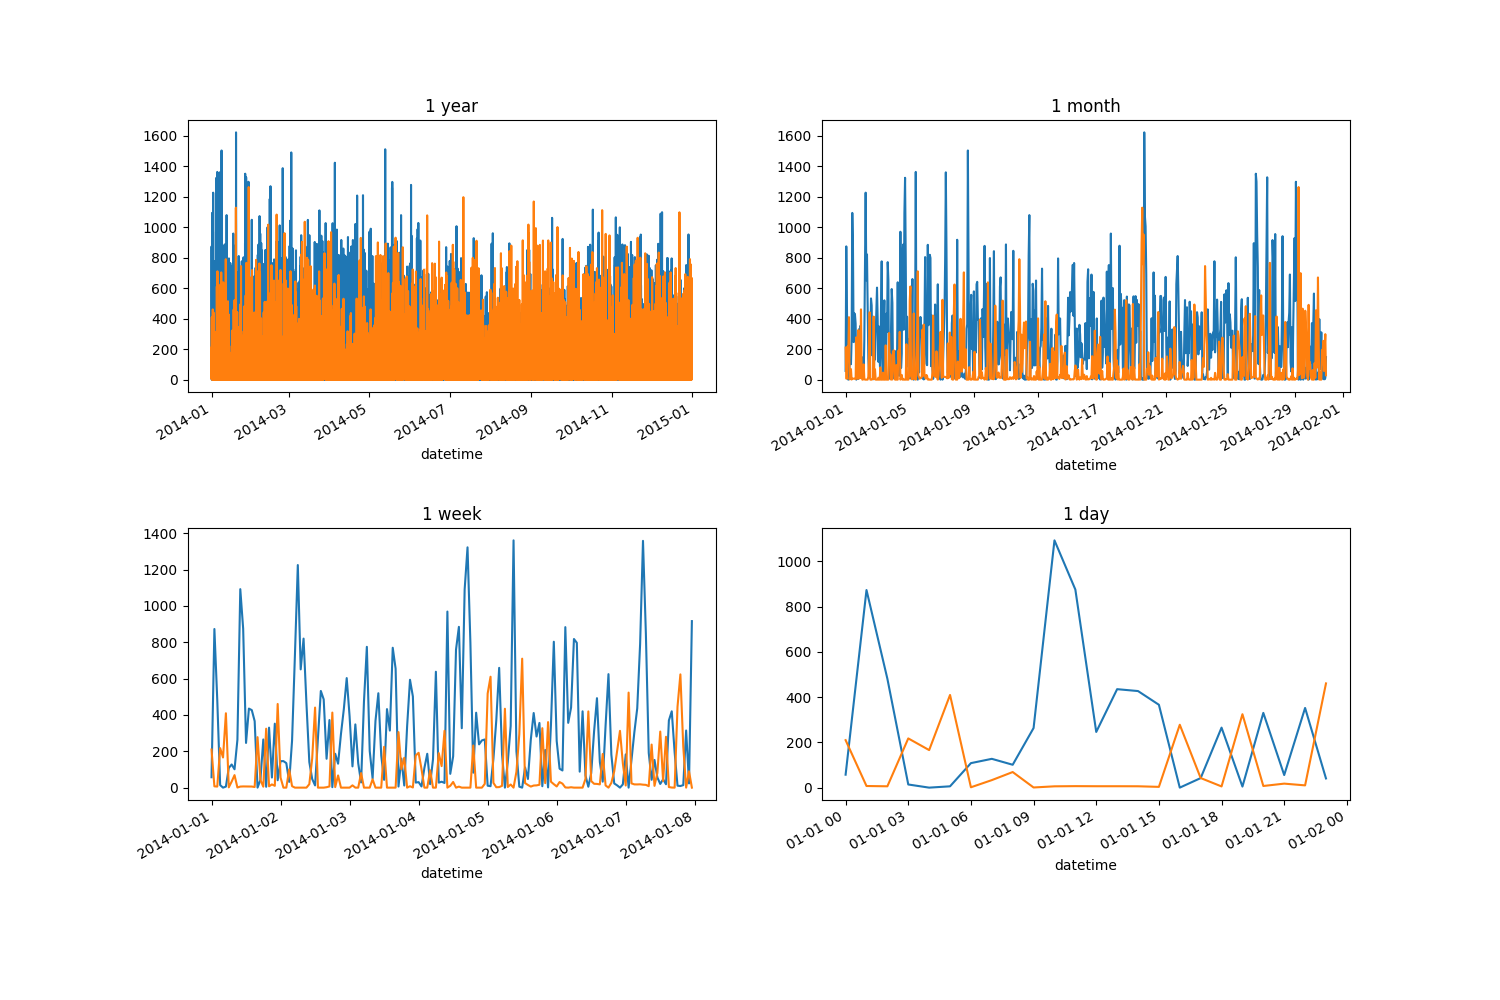
\includegraphics[width=0.7\textwidth]{plots/target_timeseries_windows.png}
  \caption{Janelas Temporais dos dados alvo}
  \label{fig:targettimeserieswindows}
\end{figure}


Da análise destas janelas temporais verificou-se claramente que ambos os atributos mantêm um comportamento tanto discreto, como linear, isto é, que ou existe algum valor, ou é zero, e se existe valor este tem comportamento linear.\par
A distribuição destes dados é claramente exponencial, o que é importante para a escolha de alguns parâmetros na modelação.\par

		
\begin{figure}[H]
  \centering
  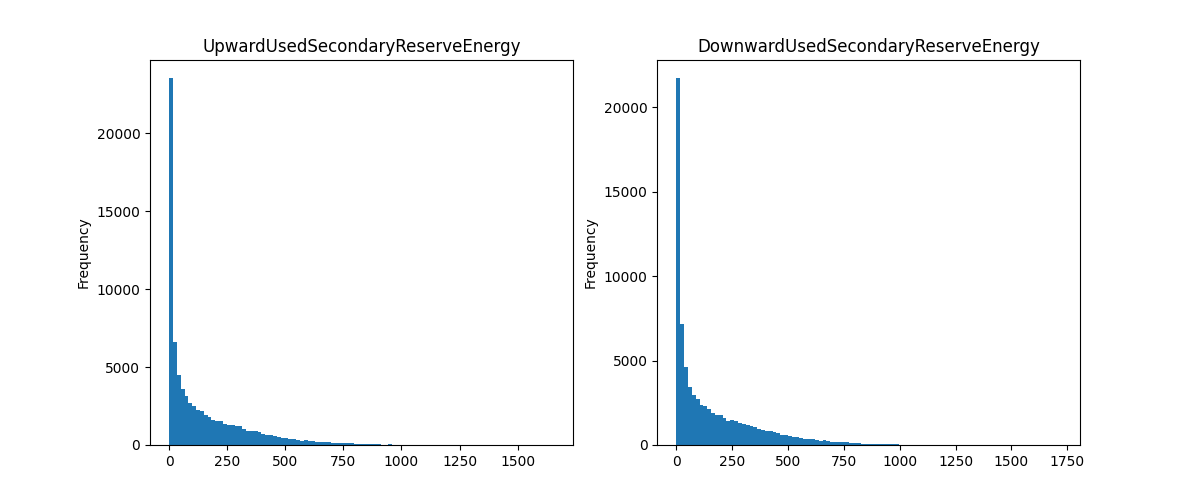
\includegraphics[width=0.6\textwidth]{plots/target_histograms.png}
  \caption{Frequência dos dados alvos}
  \label{fig:targethistograms}
\end{figure}


\paragraph{Correlações}
\text{ }  \par

Os modelos vão depender bastante de correlação entre variáveis.

Nesta secção procuramos identificar se há visiveis relações entre as variáveis, e se há relações temporais  visiveis nas colunas alvo.


\subparagraph{Correlações entre atributos}
\text{ }  \par


\begin{figure}[H]
  \centering
  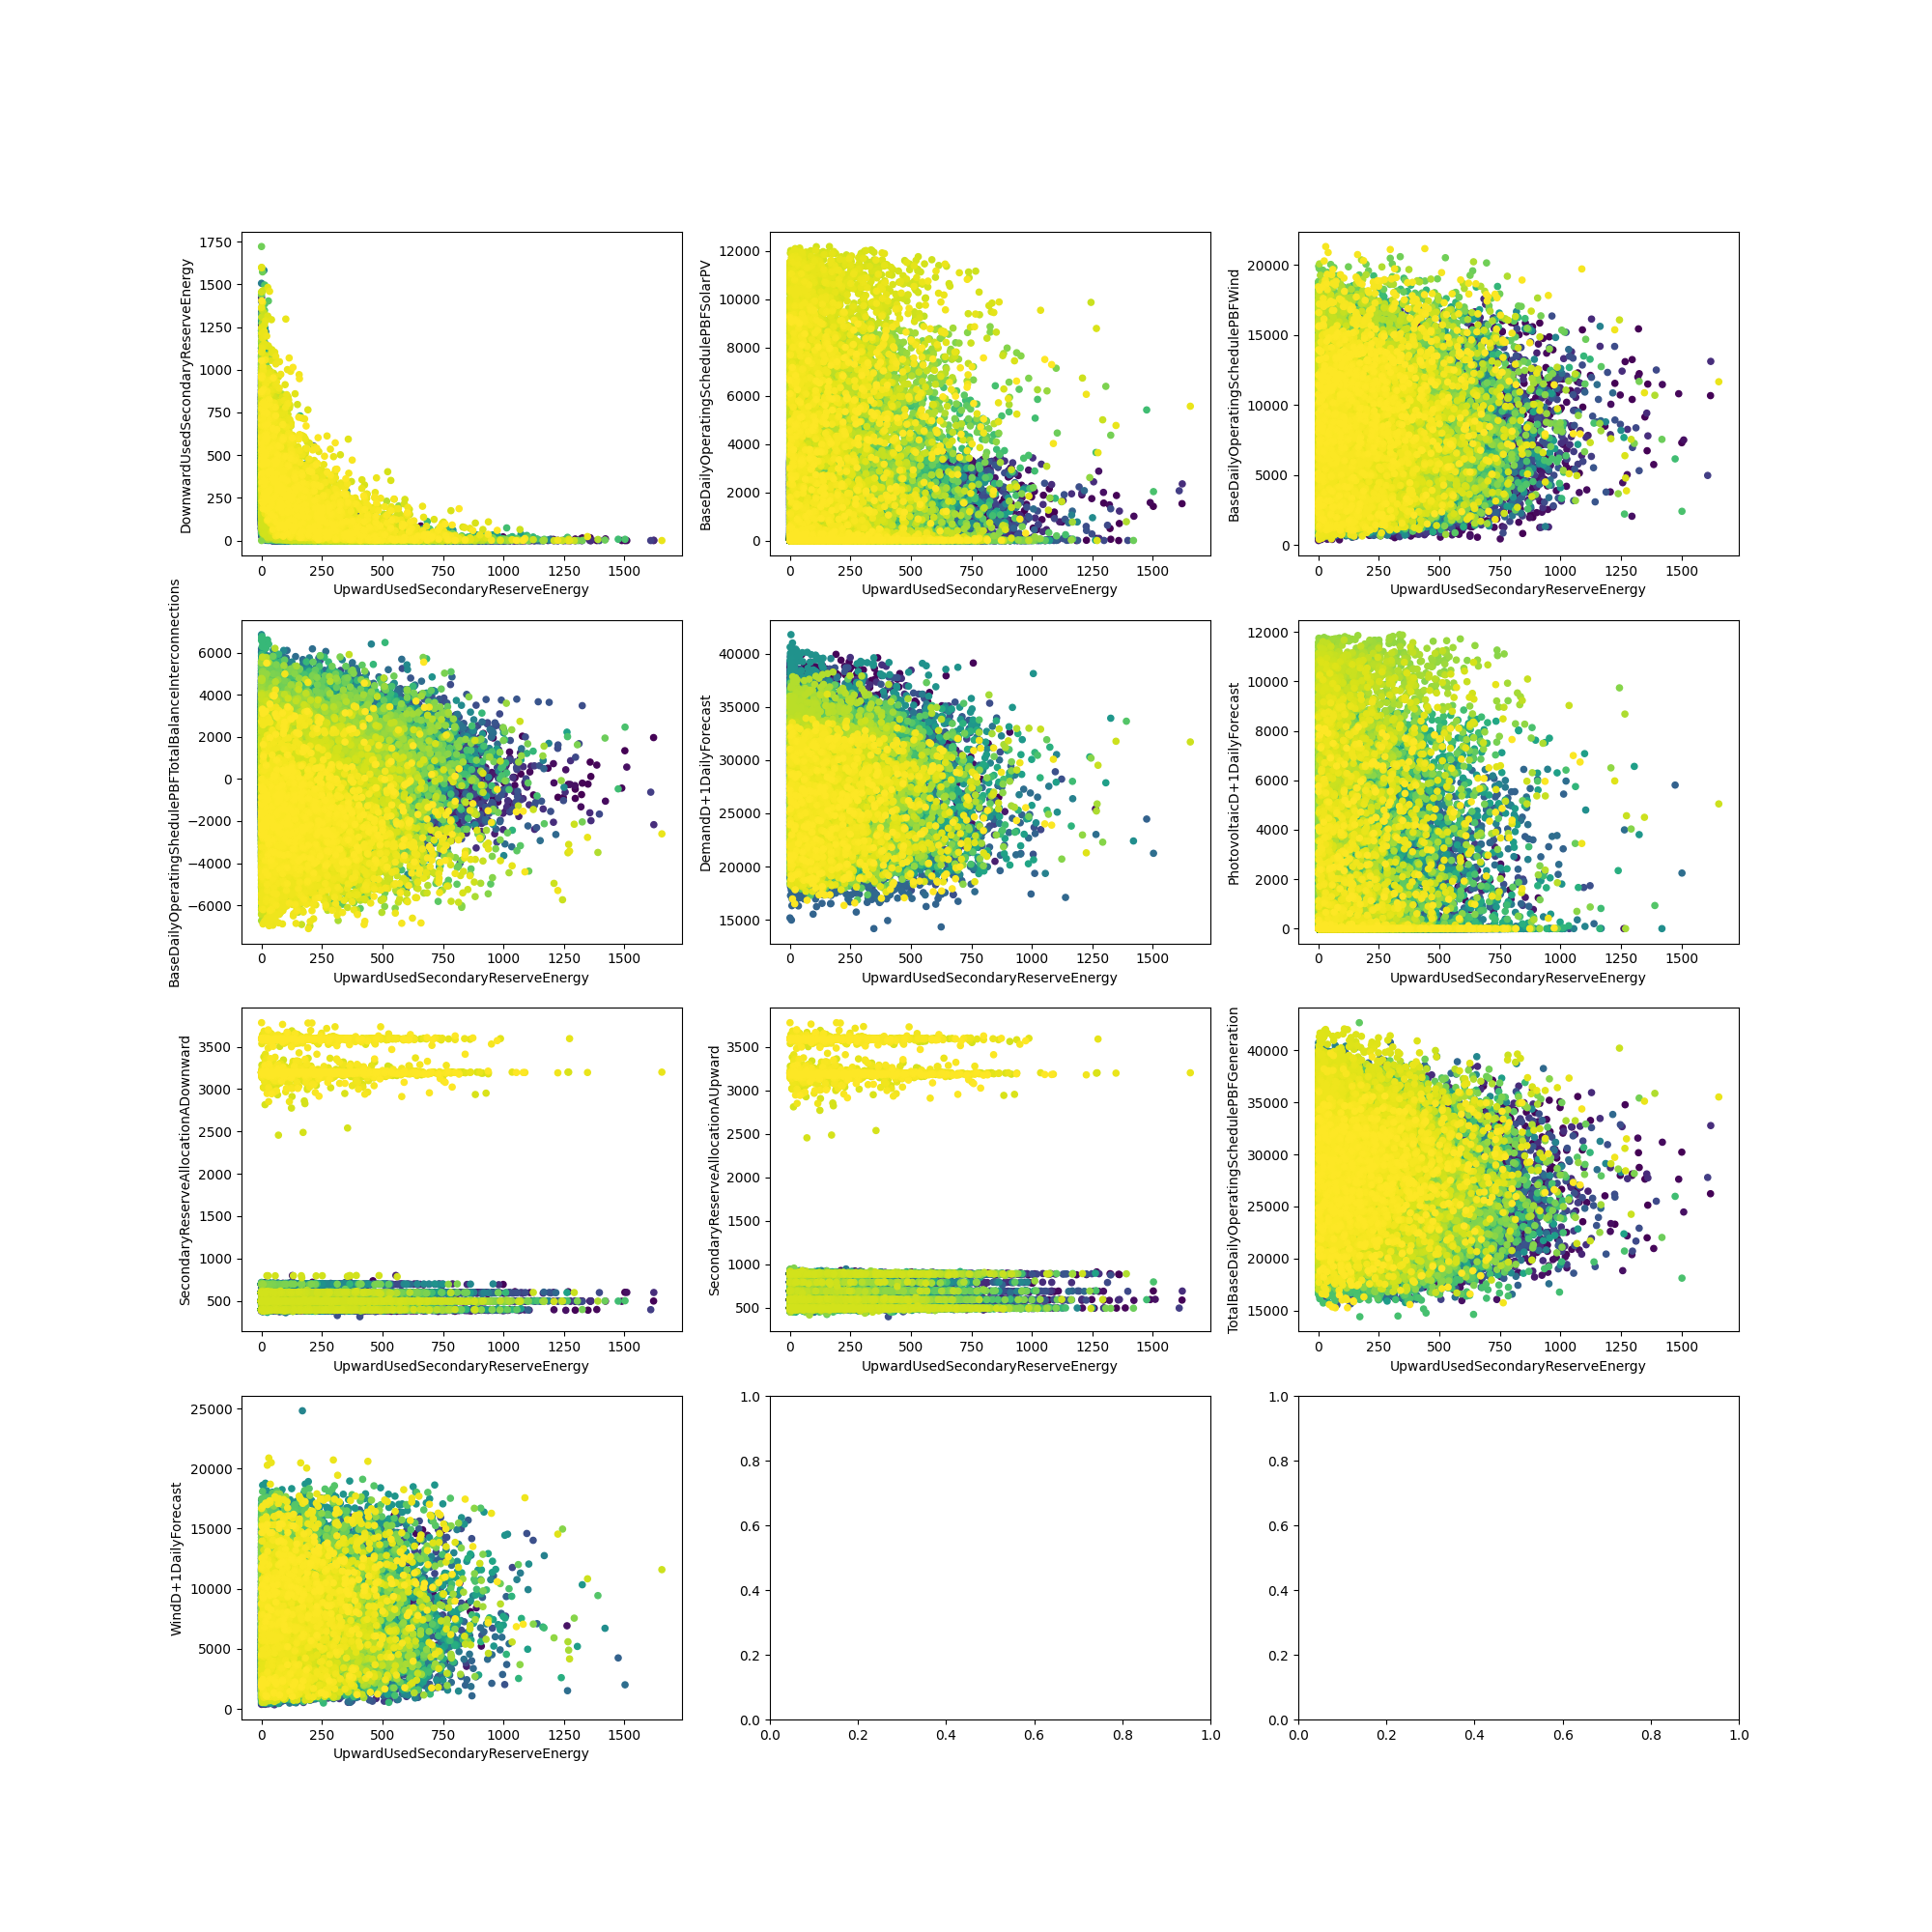
\includegraphics[width=0.90\textwidth]{plots/feature_correlation.png}
  \caption{Correlação entre atributos}
  \label{fig:featurecorrelation}
\end{figure}

Esta figura apresenta a dispersão de valores entre a energia usada, primeiras três linhas a energia para cima e as seguintes a energia para baixo, e os outros atributos presentes.\par
As correlações entre variáveis parecem muitos escassas, o que já apresenta que a previsão destes dados, usando estas variáveis, será ser um problema difícil.\par
Por norma, é feita uma seleção de atributos baseada nestas correlações, eliminando assim os atributos que ajudam menos, ou até prejudicam os modelos.\par
Seguem, \textit{infra}, os valores de correlação é possível verificar numericamente que existe muito pouca correlação entre os atributos. Onde a primeira coluna são os valores de correlação para a energia usada a subir e a segunda coluna as correlações da energia usada a descer.\par

\begin{figure}[H]
  \centering
  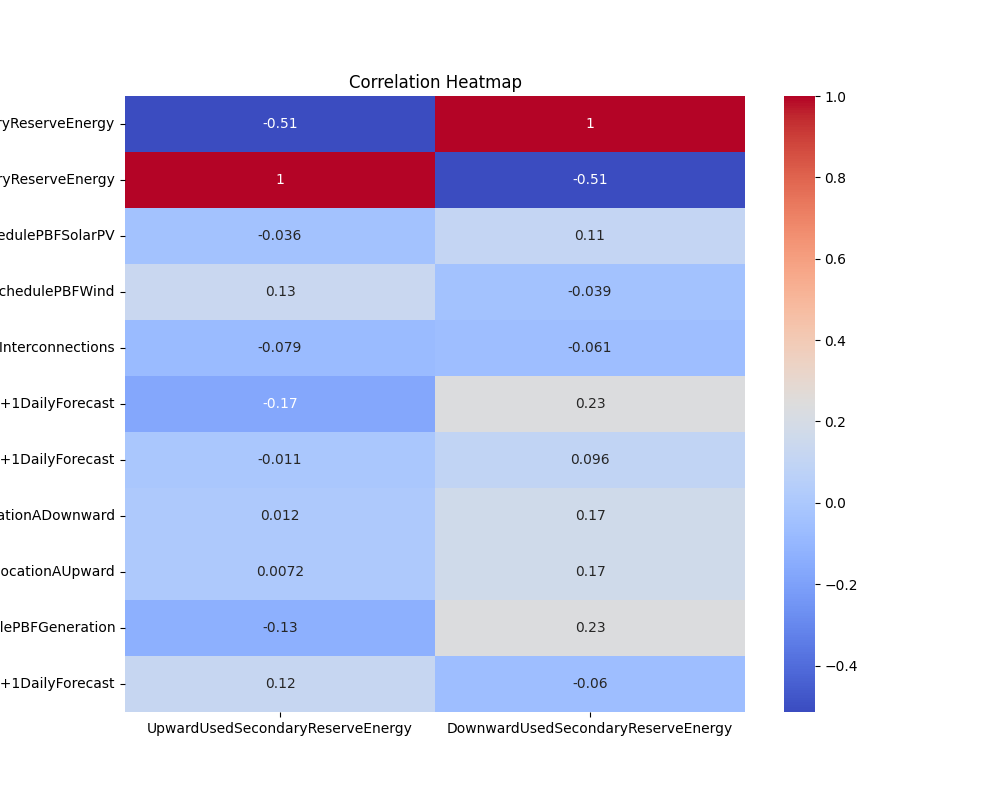
\includegraphics[width=\textwidth]{plots/correlation_heatmap.png}
  \caption{Valores de correlação entre atributos}
  \label{fig:correlationheatmap}
\end{figure}

\subparagraph{Correlações Temporais}
\text{ }  \par

\begin{figure}[H]
  \centering
  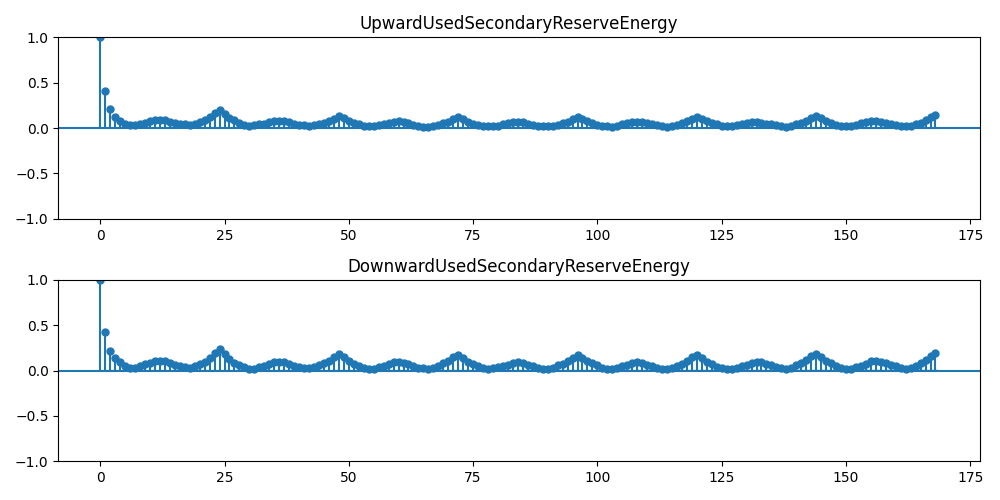
\includegraphics[width=0.75\textwidth]{plots/autocorrelation.png}
  \caption{Autocorrelação Temporal}
  \label{fig:autocorrelation}
\end{figure}

A autocorrelação, em ambos os alvos, é mais forte nas 3 horas mais próximas, e nos pontos com diferença de 12 e 24 horas.\par
É de notar que estes valores são baixos, prometendo já também uma baixa regressividade temporal.\par
Os melhores saltos temporais e suas correlações são mostradas na tabelas em baixo:\\


\begin{table}[H]
  \caption{Autocorrelação Temporal}    
  \resizebox{\linewidth}{!}{\begin{tabular}{lllllllllll}
\toprule
\midrule
\multirow[t]{2}{*}{UpwardUsedSecondaryReserveEnergy} & horas & 1 & 2 & 24 & 23 & 25 & 168 & 144 & 192 & 48 \\
 & rácio & 0.44 & 0.24 & 0.22 & 0.19 & 0.19 & 0.17 & 0.16 & 0.16 & 0.16 \\
\cline{1-11}
\multirow[t]{2}{*}{DownwardUsedSecondaryReserveEnergy} & horas & 1 & 2 & 24 & 23 & 25 & 168 & 144 & 192 & 48 \\
 & rácio & 0.43 & 0.22 & 0.25 & 0.20 & 0.19 & 0.21 & 0.19 & 0.20 & 0.19 \\
\cline{1-11}
\bottomrule
\end{tabular}
}
  \label{tab:tempcorr}
  \end{table}

Outro ponto a denotar é que os objectos não têm um comportamento completamente linear, i.e., parece existir um comportamento discreto na questão ser alocado ou não esta reservas secundárias, e caso seja alocado, aí existir alguma linearidade.\par
Logo qualquer tipo de modelação terá de resolver primeiramente este problema.\par
Da análise destas relações, é possível verificar que em termos de atributos usados será um desafio complicado para qualquer tipo de modelo.\par
No âmbito desta dissertação pretendemos verificar a qualidade das previsões usando estes mesmo atributos, pelo que, não será feita seleção dos mesmos.\par
A nível da relação temporal, a maior parte dos modelos que testaremos aplica um janela na dimensão temporal, usando todos os valores nessa janela, e aplicando os pesos nessas distâncias que mais se enquadram. Logo também não é relevante escolher apenas as distâncias temporais com maior correlação, pois os modelos farão essa pesagem.\par


